% This is samplepaper.tex, a sample chapter demonstrating the
% LLNCS macro package for Springer Computer Science proceedings;
% Version 2.20 of 2017/10/04
%
\documentclass[runningheads]{llncs}
%
\usepackage{graphicx}
\usepackage{lscape}
\usepackage{booktabs}
\usepackage{array}

\usepackage{longtable}
\usepackage[normalem]{ulem}
\usepackage{amsmath}
\usepackage[ruled,vlined]{algorithm2e}
\usepackage[table,xcdraw]{xcolor}
\usepackage{fancyvrb,newverbs}
\usepackage{hyperref}
\usepackage{float}
\usepackage{footnote}
\makesavenoteenv{tabular}

\newenvironment{compactitemize}
{ \begin{itemize}
    \setlength{\itemsep}{0pt}
    \setlength{\parskip}{0pt}
    \setlength{\parsep}{0pt}     }
{ \end{itemize}  }

\restylefloat{table}

\definecolor{cverbbg}{gray}{0.93}

\newenvironment{lcverbatim}
 {\SaveVerbatim{cverb}}
 {\endSaveVerbatim
  \flushleft\fboxrule=0pt\fboxsep=.5em
  \colorbox{cverbbg}{%
    \makebox[\dimexpr\linewidth-2\fboxsep][l]{\BUseVerbatim{cverb}}%
  }
  \endflushleft
}

\newcommand{\ctexttt}[1]{\colorbox{cverbbg}{\texttt{#1}}}
\newverbcommand{\cverb}
  {\setbox\verbbox\hbox\bgroup}
  {\egroup\colorbox{cverbbg}{\box\verbbox}}

% Used for displaying a sample figure. If possible, figure files should
% be included in EPS format.
%
% If you use the hyperref package, please uncomment the following line
% to display URLs in blue roman font according to Springer's eBook style:
\renewcommand\UrlFont{\color{blue}\rmfamily}

\begin{document}

\title{Ontologies Supporting Research-related Information Foraging Using Knowledge Graphs: Literature Survey and Holistic Model Mapping
%\thanks{This project is supported by the CSF under 98-12345S}
}
%
\titlerunning{Research-related Ontologies Survey and Holistic Model Mapping}
% If the paper title is too long for the running head, you can set
% an abbreviated paper title here
%
\author{
    Viet Bach Nguyen\inst{1}\orcidID{0000-0003-2709-3297} \and 
    Vojt\v{e}ch Sv\'{a}tek\inst{1}\orcidID{0000-0002-2256-2982} \and 
    Gollam Rabby\inst{1}\orcidID{0000-0002-1212-0101} \and
    Oscar Corcho\inst{2}\orcidID{0000-0002-9260-0753}
}
%\email{ocorcho@fi.upm.es}
%\email{nguv03@vse.cz}
%\email{svatek@vse.cz}
%\email{rabg00@vse.cz}
\authorrunning{V.B. Nguyen, V. Sv\'{a}tek, G. Rabby, O. Corcho}

\institute{University of Economics, Prague, Czech Republic \\ \email{\{nguv03,svatek,rabg00\}@vse.cz} \and Ontology Engineering Group, Universidad Politécnica de Madrid, Spain \\ \email{ocorcho@fi.upm.es}}

\maketitle              

\begin{abstract}


We carried out a literature survey on ontologies %involving 
dealing with the scholarly and research domains, %to create a comprehensive overview of available knowledge-based resources on this topic. 
with focus on modeling the knowledge graphs that would support information foraging by researchers within the different roles they fulfill during their career.
In the state of the art we identified 43 relevant ontologies, of which 34 were found sufficiently documented to be reusable. 
%that were developed specifically for use cases related to the representation of these domains. 
At the same time, based on the analysis of extensive CVs and activity logs of two senior researchers%and also taking into account some existing scholarly knowledge graphs
, we formulated a structured set of competency questions %about research-related 
that could be answered through information foraging on the web, and created a high-level conceptual model indicating the data structures that would provide answers to these questions in a holistic knowledge graph. We then studied the retrieved ontologies and mapped them on the entities and relationships from our conceptual model. We identified many overlaps between the ontologies, as well as a few missing features. Preliminary proposals for dealing with some of the overlaps and gaps were formulated.





% The scholarly/academic domain is vast and heterogeneous. As such, it presents an interesting challenge to the semantic web technologies...

% We find ontologies that can together cover our case study - everything related to researcher life

\keywords{
%academic ontologies \and bibliographic ontologies
scholarly ontology \and literature survey
\and competency question \and knowledge graph \and %ontology analysis \and %research domain \and
%research-related
information foraging %\and semantic web.
}
\end{abstract}

\section{Introduction}

On a daily basis, researchers find themselves in situations when they need to acquire %research-related
information from resources on the Web. 
The nature of such information needs differs based on the specific academic role of the researcher at the given moment, such as  that of a paper writer, event organizer, scientific evaluator, advisor of other %more junior
researchers, or %research 
project coordinator. 
Yet, many of these needs revolve around a small set of generic entity types and their relationships on which information is sought, such as people, institutions, publications, scientific venues, projects, topics, problems, arguments, or research artifacts. 
This common basis is relatively generic across research fields and makes it possible to proceed from textual search to the exploitation of structured databases on the web. 
Further, the rise of RDF-based knowledge graphs (KGs) may help overcome the rigidity of traditional database schemas; %heterogeneous 
information from independent resources could nowadays be integrated and searched with less overhead. 
%
%Generally, whatever the domain is, perhaps the greatest hindrance to wide adoption of RDF-based KG is currently their low data quality. A part of the quality issues follows from the heterogeneity of their source structures -- whether at the level of whole datasets, which may be semantically incoherent, or at the level of fine-grained knowledge items, which is typical for graphs based on crowdsourced resources such as Wikipedia.
%Another part is owing to imperfections of the transformation (ETL) process, which generates additional errors.
%Making decisions with far-reaching consequences based on such public KGs might thus still be impossible in the near future.
%However, even if we still suffer from this low data quality, such KGs can serve, in our opinion: 
%\begin{itemize}
%    \item as a first cheap (both in terms of effort and money) approximation, to be later complemented by focused analyses carried out through specialized databases with their dedicated interfaces, and
%    \item as a means of curating these specialized databases through revealing their mutual inconsistencies, which only appear when the content of such `silos' interacts within a unified KG.
%\end{itemize}
%
Yet, academic KGs spanning over many different entity types are still scarce; most published RDF datasets are only restricted to a few of these entity types, e.g., publications and their authors, paper citations, or projects and the institutions involved. Researchers who look for research-related information thus still have to either deal with multiple %structured 
databases or delve into unstructured textual search. If holistic academic KGs are to be developed to address such needs in an integrated manner, it is important to understand the currently available `eco-system' of reusable, well documented ontologies that could underlie such KGs, and point out the overlaps and %uncovered areas 
gaps in this system. While the existence of overlaps implies the need of some decision support in the choice among the overlapping ontologies, the gaps, in turn, ask for the development of new ontologies. 

Many papers published in the last two decades contained some surveys of existing scholarly ontologies, whether standalone or in comparison with a newly introduced model.
We are however unaware of either a survey or a comprehensive ontology aiming to cover the concepts referenced by the \emph{daily activities} of an (especially, senior) researcher. For such activities, a researcher takes on multiple `hats' (roles), including such that directly relate to research -- for example, not just to undergraduate education or to the general course of a working contract valid for any position and organization.
Most previous papers and models restrict the analyzed activities to `doing research' proper (methods, experiments, tools, etc.) and/or to attributes of research publications.
This is the case, e.g., for the previous standalone survey by Ruiz \& Corcho \cite{Ruiz}, focused on modeling scientific documents. 
%\cite{DBLP:journals/biomedsem/Shotton10} There are many RDF datasets on scholarly topics.... cf. Gollam's dataset survey
Similarly, the recent requirements analysis for an Open Research KG by Brack et al. \cite{Brack} is confined to the `literature-oriented' tasks of scientists.
Even the Scholarly Ontology \cite{DBLP:journals/jodl/PertsasC17}, which  comprehensively covers `scholarly practices' (using thorough modeling with the help of foundational ontologies) including entities such as projects, courses, or information resources, focuses on a use case related to scientific activities tied to experiments and paper writing.

In this paper we aim not only at updating the previous scholarly/research ontology surveys by covering some newly developed models, but, in particular, at  aligning them with a systematic analysis of information needs triggered by \emph{different research-related roles} played by researchers.
%A further distinctive feature of our research is the examination of the coverage of the proposed high-level concepts, derived from competency questions pertaining to different researcher roles, by existing ontologies, especially of those available on the web.
The information needs are expressed using \emph{high-level competency questions}, giving rise to entity type paths from which a \emph{holistic conceptual graph} was eventually built.
Entities and relationships from the graph were approximately (manually, in a lightweight manner) \emph{matched} with those of the surveyed ontologies, thus providing insights into what is covered and what is not, as well as where the overlaps are the strongest.

The main content of this paper is structured in the following way. Section \ref{section:2} describes the process of literature search through which the relevant ontologies were identified and selected. Section \ref{section:3} explains how the competency questions were formulated and  the corresponding high-level model constructed. Section \ref{section:4} presents the alignment between the model and the surveyed ontologies. Last, section  \ref{section:5} wraps up and outlines the directions for future research.


\section{Literature survey methodology and results}
\label{section:2}

The first step of our survey was to obtain a list of candidate ontologies that could potentially include entities related to researcher information needs and its context.
%The purpose of this search is to find which domain parts have been addressed in which context and what has not been addressed yet. In this section, we describe our literature review process for finding relevant artifacts for further analysis.
%
Given the fact that most ontologies and relevant projects are %potentially 
%documented 
reported in %research articles 
papers, %and presented at  conference or published in a journal within the Semantic Web area, one of the best ways to find such articles is to search in online abstract and citation databases with bibliographic information on computer science publications. Portals that have high computer science article coverage include 
a major source to be searched were high-coverage bibliographic/citation databases, of which we considered \emph{Scopus},\footnote{\url{https://www.scopus.com/}}
\emph{Web of Science}\footnote{\url{https://webofknowledge.com}}
%, DBLP%\footnote{\url{https://dblp.org/}}
%, IEEE%\footnote{\url{https://ieeexplore.ieee.org/}}
%, and the ACM Digital Library%\footnote{\url{https://dl.acm.org/}}
%. The second tier of resourceful tools are search engines such 
and \emph{Google} Scholar.\footnote{\url{https://scholar.google.com/}}
%, Microsoft Academic%\footnote{\url{https://academic.microsoft.com/home}}
%, ScienceDirect%\footnote{\url{https://www.sciencedirect.com/}}
%, CORE%\footnote{\url{https://core.ac.uk/}} 
Additionally, we also directly asked the generic \emph{Google search engine}, to also cater for ontologies not accompanied with a paper for some reason.
The different resources are complemenary.
While the (top) Google/Scholar search should lead to popular resources with many inlinks/citations, the traditional bibliographic databases primarily return respectful academic publications (even those with lower citation response) and can be searched using more sophisticated means, thus reducing the amount of noice for the subsequent manual scan of results.
While there are, obviously, a number of other possible databases to consider (such as DBLP, or the IEEE/ACM libraries), we assumed that sufficient coverage can already be obtained via the four we chose.
Finally, for directly retrieving ontologies, an obvious choice was the \emph{Linked Open Vocabularies} (LOV) portal\footnote{\url{https://lov.linkeddata.es/}} 

%For obvious reasons, Google was our first bet. 
Using Google as the initial baseline,
%With this lax and quite naive approach 
we 
%managed to find a good amount of relevant ontologies using simple terms such as
searched for the most obvious phrases only, to keep the precision acceptable: \textit{scholar/ly ontology}, \textit{academic ontology}, \textit{research/er ontology}, and \textit{bibliography/ic ontology}.
%, \textit{conference ontology}
For each Google query, we examined the first 10 pages of results, 
%(approx. 160 results). sorted by relevance. Google results represented a list of mixed resources 
which consisted in a mix of publications, projects, and actual ontology documentations. %Nevertheless, over 80\% of the listed Google results were irrelevant or duplicated based on the result title. This approach apparently requires a lot of manual evaluation and is time-consuming but the results are acceptable. In this first iteration, 
Overall we identified, this way, a total of 9 relevant ontologies. 
%which, by their titles and description, indicate high relevancy.

%\begin{itemize}
%    \item Scholarly Ontology (SO)
%    \item Scholarly Event Description Ontology (SEDE)
%    \item FOAF-Academic Ontology
%    \item Researcher Profile Ontology for Academic Environment
%    \item Ontology for Academic Program Accredication (ABET)
%    \item Academic Institution Internal Structure Ontology (AIISO)
%    \item Curriculum, Course, and Syllabus Ontology (CCSO)
%    \item SPAR Ontologies
%    \item VIVO-ISF Ontology
    %\item Informatics Research Artifact Ontology
%\end{itemize}

We then used the Google Scholar search engine with the same search terms. 
%This time we expected a significant increase in the relevancy of the search results. 
Google Scholar returned, in all cases, publications, from which %such as articles and books. Search results were enhanced with bibliographic data such as authors, publication year, venue, citations, and related articles. Among the first ten pages of Google Scholar results (approx. 160 results), the relevancy was still very low topic-wise%, but almost all results were publications
%and there was still a lot of manual checking, reading the titles and abstracts. This time, 
we  collected 5 further relevant ontologies.

%\begin{itemize}
%    \item AcademIS Ontology
%    \item Computer Science Ontology (CSO)
%    \item BIBO Ontology
%    \item CiTO Ontology
%    \item Semantic Web for Research Communities Ontology (SWRC)
%\end{itemize}

Next, we used the Scopus bibliographic database.
%, launched in 2004. is a high-quality and easy-to-use database that covers an enormous amount of bibliographic records from a large number publishers including peer-reviewed journals. 
The advantage of searching in a specialized database was the higher degree of relevance 
%and completeness because the search is focused solely on scientific publications that have mandatory indicative data used for indexing. Another advantage in searching online is that it also, in some cases, provide the user with related articles with high relevancy and citation exports. This makes it much easier and faster to find projects that make use of the mentioned ontologies.  %Keyword-based search is better compared to general-purpose search on Google because the search terms is compared against multiple meta information of the publication such as title, keywords and abstract, which are indexed. %
To make a better use of the search tools provided by Scopus, we used our search terms to search for papers by titles and keywords, while limiting the scope to the Computer Science and Engineering fields. The following snippet represents our Scopus search query, which we used for searching in the title; analogous queries were applied on the abstract and keywords:
%\begin{Verbatim}[fontsize=\small]
%    TITLE ((academic OR scholarly OR researcher OR bibliography) 
%        AND  ontology) AND (SUBJAREA("COMP") OR  SUBJAREA("ENGI")) 
%\end{Verbatim}

\begin{lcverbatim}
TITLE ((academic OR scholarly OR researcher OR bibliography) 
    AND  ontology) AND (SUBJAREA("COMP") OR  SUBJAREA("ENGI")) 
\end{lcverbatim}

The search in the titles (TITLE) yielded 57 results, the search in abstracts (ABS) yielded 2829 results, and the search in keywords (KEY) yielded 279 results, all sorted by relevance. In the case of abstract-related results, we browsed the first 10 pages (approx. 100 results). Among these results, we found a total of 22 additional ontologies.
%The following list includes several more relevant ontologies for our research:

%\begin{itemize}
%    \item Ontology for Linked Open University Data (OLOUD)
%    \item Education Standards Ontology (ESO)
%    \item Education Application Ontology (EAO)
%    \item Funding, Research Administration and Projects Ontology (FRAPO)
%    \item PLET4Thesis
%    \item Open Research Knowledge Graph Ontology (ORKG)
%    \item Ontology for Academic Department
%    \item Academic Evaluation Ontology
%    \item Ontology for Academic Context Reasoning
%    \item FRBR-aligned Bibliographic Ontology (FaBIO)
%    \item Bibliographic Reference Ontology (BiRO)
%    \item Citation Counting and Context Characterisation Ontology (C4O)
%    \item Document Components Ontology (DoCO)
%    \item Publishing Status Ontology (PSO)
%    \item Publishing Roles Ontology (PRO)
%    \item Publishing Workflow Ontology (PWO)
%    \item Scholarly Contributions and Roles Ontology (SCoRO)
%    \item DataCite Ontology
%    \item Bibliometric Data Ontology (BiDO)
%    \item FAIR* Reviews Ontology (FR)
%    \item Five Stars of Online Research Articles Ontology
%    \item OpenCitations (OC)
%\end{itemize}

Our last bibliographic database of choice was the Web of Science.  First, we searched for each term one by one. The term \textit{scholarly ontology} yielded 32 results, the term \textit{academic ontology} yielded 87 results, the term \textit{researcher ontology} yielded 182 results (all with the refinement to the `article' document type and to the `computer science and information systems' category). Next, we used a query equivalent to the one used on Scopus, for searching in the title (and, analogously, in the topic) as follows:
%\begin{verbatim}
%    TI = ((academic OR scholarly OR researcher OR bibliography) 
%        AND ontology) AND SU = (Computer Science OR Engineering)
%\end{verbatim}
\begin{lcverbatim}
TI = ((academic OR scholarly OR researcher OR bibliography) 
    AND ontology) AND SU = (Computer Science OR Engineering)
\end{lcverbatim}
This query returned 22 results for the title filter (TI) and 423 results for the topic (TS) filter. Among these results, we found 2 additional ontologies.% were found.


%\begin{itemize}
%    \item UniGrad (FOAF+SIOC extension)
%    \item Extension of the BiDO Ontology to Represent Scientific Production (BSBM)
%\end{itemize}

% http://www.scholarlydata.org/sparql/


%After a couple of search , we quickly realized that, in most cases, the resulting publications were overlapping and the number of new results was decreasing. The number of collected results each time depends on the order of chosen tools and thus does not reflect the true resourcefulness of the databases. %For that reason we did not search further on IEEE, ACM DL, Microsoft Academic, Science Direct and CORE.

Aside the keyword-based search, we also benefited from the availability of \emph{citation links} in Google Scholar, Scopus and Web of Science. 
We followed some promising incoming citation links to the papers on ontologies found so far. 
%for more papers involving ontologies that we missed during the keyword-based search. 
Using this technique, we identified 3 further ontologies.

For each ontology found through a paper reporting on it, we as much information as possible, including its metadata, source code and full texts of the referencing papers (when available). 

%\begin{itemize}
%    \item SemSur: Core Ontology for the Semantic Representation of Research Findings
%    \item Ontology for describing academic mental states
%    \item KISTI Reference \& Academic Ontology
%\end{itemize}


%Although our scope of focus is not too large, the search results could still be overwhelming in number which need proper filtering and narrowing down. 

% On the other hand, the keyword-based search might not be complete due to synonymy etc. 

Last, 
%because there is a good chance these 
we directly searched for ontologies  %listed 
on the LOV portal. We %did a thorough search on this portal and 
found a considerable amount of relevant resources using the keywords \textit{research}, \textit{academic}, \textit{scholar} and \textit{bibliography}, of which most had already been
covered by the previous bibliographic database or Google results.  
However, two new relevant ontologies were still found this way. % probably because of too generic naming:

We then used the LOV results as a referencing resource to find related literature that described them (and  possibly escaped the previous literature search), projects that used them,
%\begin{itemize}
%    \item Research Object Ontology (RO)
%    \item Common European Research Information Format Ontology (CERIF)
%\end{itemize}
as well as to complete the missing information such as the namespaces and links to the source code. 

%To reduce future problems related to both imprecision and incompleteness of a naive keyword search
To facilitate running a similar process in the future, we briefly summarize our literature search protocol for finding state-of-the-art ontology data:

\begin{enumerate}
    \item determine search engines and relevant online databases, %(based on search samples from multiple portals, results were often overlapping, so we recommend to use only Scopus which has the best tools for filtering),
    \item define search criteria for optional filtering which include the top-level field, topic or domain, and keywords including their combinations,
    \item execute initial search and iterate through an adequate amount of results,
    \item exclude duplicate articles among the initial results,
    \item manually include relevant articles based on title, keywords and abstract,
    %\item exclude articles that introduce work that are in early phase of development such as poster papers, PhD papers
    %\item exclude articles that do not mainly introduce an ontology or its usage in an applied project, [provide at least 2 examples which where excluded]
    \item since search by keyword can miss some papers, try reverse citation tracking, even if paper is weak (has not been cited many times), forward tracing, reverse tracking of citations, since a later work could include a comparison of such papers,
    \item look for ontologies in online specialized catalogs such as LOV.
\end{enumerate}

In Figure \ref{literature-review}, we provide an overview of this literature survey procedure.
\begin{figure}
\centering
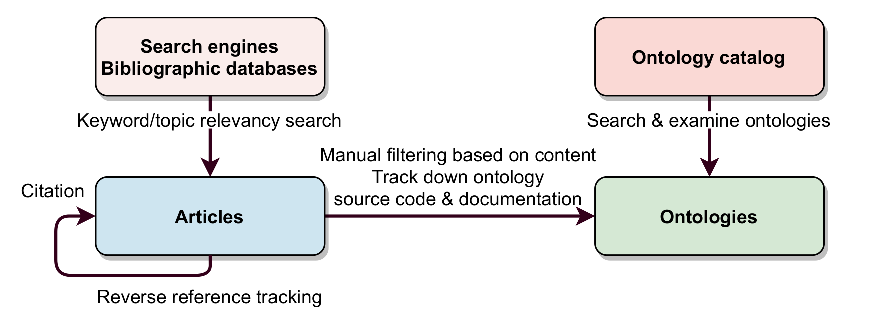
\includegraphics[width=9cm]{figures/literature-review.eps}
\caption{
    %Conceptual model for exploring literature, 
    Procedure for retrieving ontology related resources.} \label{literature-review}
\end{figure}

%The following is the list of keywords used in both literature search and LOV.
%\begin{itemize}
%    \item scholar/ly ontology,
%    \item academy/ic ontology,
%    \item research/er ontology,
    % \item publishing ontology,
    % \item referencing ontology, 
    % \item ontology for describing bibliographic resources and citations, 
    % \item ontology for describing bibliography, 
    %\item citations ontology, 
%    \item bibliography/ic ontology, 
%\end{itemize}

The result of our survey was a comprehensive table of metadata related to the ontologies. 
However, there were still some incomplete records due to unavailable or missing information.
%The next step is to examine the discovered ontologies at the 
Content-level analysis also revealed some ontologies that were likely irrelevant for practical information search, e.g., an `Ontology for describing academic mental state'. 
From the totality of 43 ontologies found, we thus eventually chose 34 for which 1) we deemed the availability of source code and/or metadata sufficient for effective reuse, and 2) the ontology content was indeed relevant to researcher information needs.
Table \ref{tab:research-related-ontologies}
%and \ref{tab:research-bib-related-ontologies} 
shows the final list of ontologies\footnote{Some acronyms in this table are unofficial, e.g. OAD or RPO, and are only introduced for convenient referencing within this research.} used in our subsequent analysis.

\begin{table}[]
\centering
\caption{Research-related ontologies}
\label{tab:research-related-ontologies}
\begin{tabular}{llr}
\toprule
\textbf{Acronym} & \textbf{Name}                                                                             \\ \midrule
SO            & Scholarly Ontology & \cite{DBLP:journals/jodl/PertsasC17}                                      \\ \midrule
OLOUD         & Ontology for Linked Open University Data & \cite{10.12700/APH.14.4.2017.4.4}                   \\ \midrule
VIVO          & VIVO-ISF Ontology & \cite{DBLP:series/synthesis/2012Borner}                                    \\ \midrule
CCSO          & Curriculum, Course, and Syllabus Ontology & \cite{DBLP:conf/esws/KatisKAV18}                   \\ \midrule
AIISO         & Academic Institution Internal Structure Ontology & \cite{DBLP:conf/incos/KalemiM11}            \\ \midrule
FRAPO         & Funding, Research Administration and Projects Ontology & \cite{Frapo}                          \\ \midrule
ORKG          & Open Research Knowledge Graph & \cite{DBLP:conf/kcap/OelenJFSA19}                              \\ \midrule
ESO \& EAO    & Education Standards \& Education Application Ontology & \cite{DBLP:conf/semweb/RashidM18}      \\ \midrule
SEDE          & Ontology for Scholarly Event Description & \cite{DBLP:journals/jis/JeongK10}                   \\ \midrule
OAD           & Ontology for Academic Department & \cite{An:OAD}                                               \\ \midrule
AcademIS      & AcademIS Ontology & \cite{DBLP:conf/pci/TriperinaST13}                                         \\ \midrule
CSO           & The Computer Sciene Ontology & \cite{DBLP:conf/semweb/SalatinoTMOM18}                          \\ \midrule
BIBO          & The Bibliographic Ontology & \cite{bibo}                                                       \\ \midrule
FOAF-Academic & FOAF-Academic Ontology & \cite{DBLP:conf/incos/KalemiM11}                                      \\ \midrule
%PLET4Thesis   & PLET4Thesis & \cite{DBLP:conf/icetc/Tapia-LeonSCL17}                                           \\ \midrule
SemSur        & Semantic Survey Ontology & \cite{DBLP:conf/i-semantics/FathallaVA018}                          \\ \midrule
RO            & Research Object Ontology & \cite{DBLP:journals/corr/BelhajjameZGHPCGBKG14}                     \\ \midrule
SWRC          & Semantic Web for Research Communities & \cite{DBLP:conf/epia/SureBHHO05}                       \\ \midrule
ABET          & Ontology for Academic Program Accreditation & \cite{10.14569/IJACSA.2016.070717}               \\ \midrule
RPO           & Researcher Profile Ontology for the Academic Environment & \cite{DBLP:conf/cvc/BravoRC19}      \\ \midrule
%IRAO          & Informatics Research Artifacts Ontology                                                     \\ \midrule
CERIF         & Common European Research Information Format Ontology & \cite{DBLP:journals/datascience/Jorg10} \\ \midrule
FaBiO         & FRBR-aligned Bibliographic Ontology & \cite{DBLP:journals/ws/PeroniS12}                        \\ \midrule
CiTO          & Citation Typing Ontology & \cite{DBLP:journals/ws/PeroniS12}                                   \\ \midrule
BiRO          & Bibliographic Reference Ontology & \cite{DBLP:conf/esws/IorioNPSV14}                           \\ \midrule
C4O           & Citation Counting and Context Characterisation Ontology & \cite{DBLP:conf/semweb/OsbornePM14}  \\ \midrule
DoCO          & Document Components Ontology & \cite{DBLP:journals/semweb/ConstantinPPSV16}                    \\ \midrule
PSO           & Publishing Status Ontology & \cite{DBLP:conf/i-semantics/PeroniSV12}                           \\ \midrule

%\\ \bottomrule

%\end{tabular}
%\end{table}

%\begin{table}[]
%\caption{Research-related ontologies}
%\label{tab:research-bib-related-ontologies}
%\begin{tabular}{ll}
%\toprule
%\textbf{Acronym} & \textbf{Name}   \\ \midrule
PRO           & Publishing Roles Ontology & \cite{DBLP:conf/i-semantics/PeroniSV12}                            \\ \midrule
PWO           & Publishing Workflow Ontology & \cite{DBLP:journals/semweb/GangemiPSV17}                        \\ \midrule
SCoRO         & Scholarly Contributions and Roles Ontology & \cite{Scoro}                                      \\ \midrule
DataCite      & DataCite Ontology & \cite{DataCite_Ontology}                                                   \\ \midrule
BiDO          & Bibliometric Data Ontology & \cite{tapia2019extension}                                         \\ \midrule
FiveStars     & Five Stars of Online Research Articles Ontology & \cite{DBLP:journals/dlib/Shotton12}          \\ \midrule
FR            & FAIR* Reviews Ontology & \cite{Fair}                                                           \\ \midrule
%BSBM          & Extension of the BiDO Ontology to Represent Scientific Production & \cite{tapia2019extension}  \\ \midrule
OCO           & OpenCitations Ontology & \cite{DBLP:journals/qss/PeroniS20}

\\ \bottomrule

\end{tabular}
\end{table}



% 

\medskip
\noindent \textbf{Description of ontologies}

\medskip
\noindent \textbf{OLOUD-BASE} \& \textbf{OLOUD-LOC}. \cite{10.12700/APH.14.4.2017.4.4} The objectives of the OLOUD ontology is to support the development and publishing of Linked Open University Datasets and the applications built on the top of these Open Datasets. OLOUD contains classes and properties to describe Organizations, People, their Roles and Publications, Subjects, Courses and other Events and their temporal and spatial description. The ontology is divided into two connected modules: 1. OLOUD-BASE is the main module describing all the university related concepts and uses the prefix \texttt{oloud}, 2. OLOUD-LOC module provides the indoor location and navigation features and uses the prefix \texttt{loc}.

\medskip
\noindent \textbf{VIVO}. \cite{DBLP:series/synthesis/2012Borner} An ontology of academic and research domain, developed in the framework of the VIVO project. It represents researchers in the context of their experience, outputs, interests, accomplishments, and associated institutions.

\medskip
\noindent \textbf{SWRC}. \cite{DBLP:conf/epia/SureBHHO05} An ontology for modeling entities of research communities such as persons, organisations, publications (bibliographic metadata) and their relationship.

\medskip
\noindent \textbf{ABET}. \cite{10.14569/IJACSA.2016.070717} Ontology of Accreditation Board of Engineering and Technology Process. It helps faculty  or  curriculum  committees  avoid  over  mapping  or  under mapping students' outcomes.

\medskip
\noindent \textbf{CCSO}. \cite{DBLP:conf/esws/KatisKAV18} This Ontology aims to provide data model for describing the subjects of Curriculum, Course and Syllabus in Higher education. Using this ontology, syllabus items can be effectively described and annotated enabling intelligent systems to support teaching and learning by offering automated services like syllabus semantic searching, matching and interlinking, syllabus recommendation and evolution.

\medskip
\noindent \textbf{FOAF-Academic}. \cite{DBLP:conf/incos/KalemiM11} A Vocabulary for the Academic Community. This ontology helps the academic community in saying anything about their achievements, their qualifications, activities and the communities that are near to them.

\medskip
\noindent \textbf{AIISO}. \cite{DBLP:conf/incos/KalemiM11} The Academic Institution Internal Structure Ontology (AIISO) provides classes and properties to describe the internal organizational structure of an academic institution.

\medskip
\noindent \textbf{ESO} \& \textbf{EAO}. \cite{DBLP:conf/semweb/RashidM18} Education Application Ontology and Education Application Ontology are used to simplify lesson planning for teachers, providing support for students by linking relevant resources, and providing a potential terminology for use in a lingua-franca for communicating with multiple communities about education components.

\medskip
\noindent \textbf{PLET4Thesis}. \cite{DBLP:conf/icetc/Tapia-LeonSCL17} The PLET4Thesis ontology is designed in order to organise the process of thesis development using the elements required to create a PLE (personal leaning environment).  Designed to guide thesis students in the construction of their PLE.

\medskip
\noindent \textbf{ORKG}. \cite{DBLP:conf/kcap/OelenJFSA19} The Open Research Knowledge Graph Ontology is used for comparing research contributions in a scholarly knowledge graph.

\medskip
\noindent \textbf{Researcher Profile Ontology}. \cite{DBLP:conf/cvc/BravoRC19} This ontology is designed specifically to represent academic contexts at a public university. It supports the representation of researcher profiles in a given academic environment.

\medskip
\noindent \textbf{IRAO}. Used to describe research artifacts in research, including authorship, evolution, etc.

\medskip
\noindent \textbf{CERIF}. \cite{DBLP:journals/procedia/JorgLK12} The Common European Research Information Format (CERIF) Ontology Specification provides basic concepts and properties for describing research information as semantic data. This document contains a friendly description of the Common European Research Information Format (CERIF) Ontology developed by EuroCRIS.

\medskip
\noindent \textbf{RO}. \cite{DBLP:journals/ws/Belhajjame0GGHP15} The Research Object Ontology provides basic structure for the description of aggregated resources and the annotations that are made on those resources.




%add by gollam rabby
% start

\medskip
\noindent \textbf{FaBiO}. FaBiO\cite{DBLP:journals/ws/PeroniS12} is an ontology applied for describing the entities that are published or undeniably publishable works (e.g. journal articles, conference papers, books), that contain or suggest bibliographic references. It also covers data sets, web pages, blogs, computer algorithms, formal specifications and vocabularies, experimental protocols, legal records, technical and commercial reports, governmental papers and similar publications, and also anthologies, catalogs, and corresponding collections. FaBiO has been developed to overcome any restriction to the classes and the domains with ranges of its properties. It is flexible and it has a superb advantage of allowing itself to be used side by side with other models.

\medskip
\noindent \textbf{CiTO}. CiTO\cite{DBLP:journals/biomedsem/Shotton10} is an ontology that allows characterization of the character or type of citations, both factually and rhetorically. Properties and consequently their inverses could even be classified as rhetorical and/or factual, with the rhetorical properties being grouped in three sets: positive, informative (neutral), or negative. The domain and range constraints from this thing and also properties aren't defined, so this ontology is easily integrable with other ontology models, like FaBiO. Two other ontologies are defined explicitly for describing specific aspects of CiTO, the first one is called Functions of Citations Ontology (FOCO) and the other one is called CiTO to Wordnet Ontology (C2W).

\medskip
\noindent \textbf{BiRO}. BiRO\cite{DBLP:conf/esws/IorioNPSV14} is an ontology designed to define the bibliographic records, bibliographic references, and their compilation into bibliographic collections and lists. This ontology also uses an OWL-based definition of the FRBR model\cite{bowen2011frbr} to identify the bibliographic references and their compilation into ordered bibliographic lists.

\medskip
\noindent \textbf{C4O}. C4O\cite{DBLP:conf/semweb/OsbornePM14} also provides the ontological structures which permit to record the amount of in-text citations, alongside their textual citation contexts and also the number of citations a cited entity has received globally on a specific date. It is also useful to explain how references are utilized in the citing paper. 

\medskip
\noindent \textbf{DoCO}. DoCO\cite{DBLP:journals/semweb/ConstantinPPSV16} is an ontology that organizes structured vocabulary from written document components following both structural (e.g. block, inline, paragraph, section, chapter) and rhetorical (e.g. introduction, discussion, acknowledgments, reference list, figure, appendix) options. It also imports the Pattern Ontology which describes the structural patterns, and therefore the Discourse Element Ontology (DEO), which was developed with DoCO to explain the rhetorical components. DoCO also defines hybrid classes to describe elements that are both structural and rhetorical in nature, like paragraph, section, or list. In addition, it aligned with the SALT Rhetorical Ontology and therefore the Ontology of Rhetorical Blocks (ORB).


\medskip
\noindent \textbf{PSO}. PSO\cite{DBLP:conf/i-semantics/PeroniSV12} ontology is designed and developed according to the TVC pattern, to characterize the publication status (e.g. draft, submitted, under review, etc.) of documents at every stage of the publishing process. Documents hold a specific status at a specific time as an immediate consequence of a particular event. Other pre-existing ontologies describing the status of documents (e.g. BIBO), rely on the specific property links but PSO prevents a correct description of scenarios.  

\medskip
\noindent \textbf{PRO}. PRO\cite{DBLP:conf/i-semantics/PeroniSV12} is an ontology that also uses the TVC pattern for characterization of the roles of agents (e.g. people, corporate bodies, and computational agents) within the publication process. Most of the time, the agents are authors, editors, reviewers, publishers, or librarians. It defines publishing roles as crucial as providing an entire description of a scholarly resource like a paper or a dataset.  

\medskip
\noindent \textbf{PWO}. PWO\cite{DBLP:journals/semweb/GangemiPSV17} is an ontology with two main classes called Workflow and Step, used for describing the steps of the workflow related to the publication of a document or other publication entity.

\medskip
\noindent \textbf{SCoRO}.SCoRO\cite{Scoro} is the Scholarly Contributions and Roles Ontology (CERIF-compliant ontology) for describing the contributions of authors, publishers, students, and research administrators. It is possibly used in those organizations where they're members with concerning projects, research investigations, and other academic activities focusing on scholarly journal articles and other outputs.

\medskip
\noindent \textbf{FRAPO} FRAPO\cite{Frapo} is the Funding Research Administration and Projects Ontology, which also uses a CERIF-compliant ontology for describing administrative information concerning grant funding and research projects. It also imports FOAF for characterizing people. It is mostly used for the characterization of grant applications, funding bodies, research projects, project partners, etc (the type of data stored in Current Research Information Systems (CRIS)). It also can be described as other sorts of projects, for instance, building projects and academic projects.

\medskip
\noindent \textbf{DataCite}. The main intent of the DataCite\cite{DataCite_Ontology} Ontology is to stock a versatile mechanism to prescribe the identifier for bibliographic resources and related entities. it also allows supplying a link between a resource and therefore the document describing its metadata utilizing CiTO, using the property citesAsMetadataDocument, and FaBiO, through the category of MetadataDocument. Additionally, to those entities, the DataCite Ontology provides appropriate classes and properties to specify the actual scheme followed to create the resource metadata exemplified within the metadata document.


\medskip
\noindent \textbf{BiDO}. BiDO\cite{tapia2019extension} developed a well-known model for enabling the classification of authors and journals consistent with bibliometric data, also share and reuse the data during a different context. The core module of the ontology allows one to explain any entity and therefore the related bibliometric data at a particular time and consistent with a particular agent. BiDO consists of three different modules and people are Standard bibliometric measures, Research career categories, and Review measures.

\medskip
\noindent \textbf{FiveStars}. To measure the standard of any multidimensional online journal a five stars' constellation like approach is followed by Five Stars of Online Journal Articles. The properties which are considered as stars are review quality, accessibility, content enrichment, availability of datasets and the machine-readable metadata. Articles of the online journals are evaluated based on these properties to enhance research quality and communications. This five star based conceptual framework is undoubtedly very helpful for researchers and other personnel's associated with journal publishing.\cite{DBLP:journals/dlib/Shotton12}

\medskip
\noindent \textbf{FAIR}.  FAIR \cite{Fair} is a review ontology (FR) that identifies a group of classes, properties, and axioms for describing research reviews as semantic objects and also reuse standard existing vocabularies by utilizing ontology engineering techniques.


\medskip
\noindent \textbf{BSBM}. BSBM\cite{tapia2019extension} is an enhancement of the BiDO Ontology, particularly BiDO Standard Bibliometric Measures.


\medskip
\noindent \textbf{OC}. The OpenCitations Data Model (OCDM)\cite{DBLP:journals/corr/abs-1906-11964} is the metadata model used for the stored information all together in the OpenCitation datasets. OCDM also allows us to record information about published bibliographic resources,https://www.overleaf.com/project/5ebbc2be39c6e30001174487 possible resource embodiments, bibliographic references, responsible agents, roles, citations, and external identifiers.


\medskip

 %end

\section{
%Constructing 
%natural 
%the concept hierarchy and relationships
Roles, competency questions and conceptual model}

\label{section:3}

As mentioned, our starting point for examining the required coverage for scholarly knowledge graphs were the researcher needs associated with their research-related activities.
Our approach is thus more `human-centric', compared to `data-centric' approaches to scholarly KG requirement analysis, which primarily look at what is already available in structured databases and KGs.

We started with identifying the \emph{roles} fulfilled by researchers and entailing information foraging from external sources. 
For this purpose, the two senior co-authors (VS and OC) went through their comprehensive CVs and/or daily activity log, and distilled from the activities and achievements a set of distinct roles. 
%Our model is based solely on competency questions. Hence our approach is to start by identifying types of stakeholders interested in the construction and/or use of the knowledge graph.  %Researchers can play different roles in different contexts throughout their career repeatedly, hence w
The following roles (partially grouped, for brevity) have been identified:

\begin{itemize}
    \item Researcher (general) - researching and publishing
    \item Leader of a research group  (or of a more formal unit such as a Department)
    \item Advisor (of PhD students, or generally, more junior colleagues)
    \item Event organizer / Volume editor / Journal board member
    \item Evaluator of publications, researchers, organizations/groups, projects, and funding programs
    \item Research project proposer / manager
    \item Industry transfer mediator / recruiter.
\end{itemize}

%At first, we also included entities of the more academic/educational context such as \textit{teacher}, \textit{student}, and of the more industrial and public context such as \textit{journalist}, because there exist competency questions involving them. In the end, we have decided to limit our scope to focus mainly on the domain of research due to extensive and unnecessary complexity. However, it is still a considerable possibility to include these concepts and extend our model to achieve a broader and more comprehensive ecosystem.

%After having identified the significant roles of a researcher, our next step is to identify what kinds of applications could make use of public scholarly knowledge graphs with the underlying ontologies based on our model. This is to create a holistic presumption of which competency questions should arise. The knowledge base could contain basic data about individual researchers and their work, which is trivial and could be solved in many conventional ways. Such applications include generation of researcher CVs, summarized dashboards of academic organizations or research groups, basic search for researchers and research projects. However, the advantages of modeling a model of thoroughly interconnected concepts using ontologies is the ability to exploit the linkage and relationships between many data instances as well as making use of reasoners to derive facts. This opens up and leverages a wide range of potential use cases for applications which can provide richer, more relevant and extensive experiences for users in many context. Such applications include faceted research lookup, smart research recommender, research topic aggregator \& statistical analysis, research data miner, researcher timelines, research contributions referencer.

For each researcher role, we formulated several verbal \emph{competency questions} (CQs) and equipped them with \emph{paths} of high-level concepts and relationships whose instantiations should  provide answers to the questions in a hypothetical KG. An example of path is \texttt{RESEARCHER - ORGANIZATION - EVENT}. This way, we created a set of paths from which we then constructed a holistic, highly abstract \emph{conceptual model} presented in Figure \ref{relationship-model}. We also gathered the terms in these paths into a separate collection. These terms were later put into a logical hierarchy, as shown in Figure \ref{natural-concept-hierarchy}. To reduce the complexity of the conceptual model, we only show ten top-level terms in it.
In Table \ref{tab:competency-questions} we showcase several chosen CQs and associated paths.
(To demonstrate the wider scope of the conceptual model, we omit the roles of `general' researcher and publication writer, as these have been the main focus of most previous initiatives surveying  scholarly ontologies/KGs.
They are however also part of our complete CQ set.)%, which is available on our research repository\footnote{\url{https://github.com/nvbach91/iga-knerd}})

\begin{table}[]
\caption{Examples of high-level competency questions and entity type paths}
\label{tab:competency-questions}
\begin{tabular}{|p{6cm}|p{6cm}|}
\hline
%\multicolumn{2}{|l|}{\textbf{Researcher CQ}}                                                                                                                                                                                                                                                           \\ \hline
%What has been researched / written on this topic?                                                                                                     & Topic - Project - Publication                                                                                                                  \\ \hline
%Who already had projects on this or similar topic?                                                                                                    & Researcher - Project - Topic - Topic                                                                                                           \\ \hline
%Who cites my publications?                                                                                                                            & Researcher - Publication - Publication                                                                                                         \\ \hline
\multicolumn{2}{|l|}{\textbf{Research Group Leader / Advisor CQ}}                                                                                                                                                                                                                                      \\ \hline
What positions (in projects, or general) in other organizations may attract junior researchers as an alternative to working in my group?                                            & $\bullet$ Topic - Project - Organization \newline $\bullet$ Topic - Position - Organization                                                                                                                     \\ \hline
\multicolumn{2}{|l|}{\textbf{Research Event Organizer / Volume Editor / Journal Board Member CQ}}                                                                                                                                                                                                      \\ \hline
Who should I invite as keynote speaker or reviewer (based on thematic relevance, research quality, and history of engagement in this or similar events)?       & $\bullet$ Topic - Publication - Researcher - \newline Assessment \newline $\bullet$ Topic - Researcher - Assessment \newline $\bullet$ Publication Venue - Publication - \newline Researcher - Assessment       \\ \hline
\multicolumn{2}{|l|}{\textbf{Evaluator of publications CQ}}                                                                                                                                                                                                                                            \\ \hline
What has been researched / written on the topic this publication deals with?                                       & $\bullet$ Publication - Topic - Publication \newline $\bullet$ Publication - Topic - Project                                                                               \\ \hline
What has the author previously published on this topic? What is the overlap with the current paper?                                                   & $\bullet$ Publication - Researcher - Publication - Topic                                                                                                 \\ \hline
How does the paper comply with the standard criteria of scientific writing?  
What argument is used by an author or a reviewer in a publication/review? & $\bullet$ Publication - Assessment\newline
$\bullet$ Publication - Review - Argument

\\ \hline
\multicolumn{2}{|l|}{\textbf{Evaluator of researchers CQ}}                                                                        \\ \hline
How important are the venues where the researcher publishes?                                                                                         & $\bullet$ Researcher - Publication Venue - \newline Assessment                                                                                                    \\ \hline
How much technology transfer activity (to industry) does a researcher do?                                                                             & $\bullet$ Researcher - Organization                                                                                                                      \\ \hline
%\textbf{Evaluator of academic institutions / groups}                                                                                                  &                                                                                                                                                \\ \hline
%How many publications, and of what kinds, has the institution published?                                                                              & Organization - Researcher - Publication                                                                                                        \\ \hline
%How much scientific outreach is done by researchers in the institution? (E.g., events and publications for the general public)                        & Organization - Event \newline Organization - Researcher - Publication                                                                                  \\ \hline
\multicolumn{2}{|l|}{\textbf{Evaluator of projects CQ}}                                                                \\ \hline
How topical are the goals of the project, in terms of problems addressed? Do people often write on these problems? Are they encouraged by funding programs?          &  $\bullet$ Project - Goal/Problem - Publication - \newline Researcher\newline                     $\bullet$ Project - Goal/Problem - Program                                        \\ \hline
\multicolumn{2}{|l|}{\textbf{Project proposer CQ}}          \\ \hline
                              What are the preferred topics of the program/call? What are the topical problems in the field? &
$\bullet$ Program - Topic - Problem
                      \\ \hline
Who has experience with previous projects in the chosen program?
&
$\bullet$ Program - Project - Researcher 
                      \\ \hline
What partners should be invited for such a kind of project, based on the problem addressed?
&
$\bullet$ Problem - Publication - Researcher - \newline Organization\newline
$\bullet$ Problem - Method - Researcher - Organization
                      \\ \hline
What is the usual budget of projects in this program?
&
$\bullet$ Program - Project
                         \\ \hline
%\multicolumn{2}{|l|}{\textbf{Evaluator of programs CQ}}                                                                                                                                                                                                                                                \\ \hline
%How successful are the projects funded by this program?                                                                                               & Funding Program - Project - Publication - Publication Venue - Assessment; Funding Program - Project - Method/Patent; Funding Program - Project \\ \hline
%\multicolumn{2}{|l|}{\textbf{Project proposer CQ}}                                                                                                                                                                                                                                                     \\ \hline
%What are the preferred topics of the program/call? What are topical problems in the field?                                                            & Funding Program - Topic                                                                                                                        \\ \hline
%Who has experience with previous projects in the chosen program?                                                                                      & Funding Program - Project - Researcher                                                                                                         \\ \hline
\multicolumn{2}{|l|}{\textbf{Industry transfer promotor CQ}}                                                                                                                                                                                                                                           \\ \hline
Which company or other organization is active in the given field, as a potential transfer target?                                                     & $\bullet$ Project - Topic - Organization                                                                                                                 \\ \hline

\end{tabular}
\end{table}

%We then proceeded to composing a list of glossary terms of research-relevant concepts and constructing their natural hierarchy based on interviewing and examining activity journals of two senior researchers who have gone through most of their research and pedagogic career. 
The hierarchy in Figure \ref{natural-concept-hierarchy} shows six of the top-level concepts, further broken down to subtypes. The scope and purpose of each concept are as follows:
\begin{itemize}
    \item The \textit{Topic} concept may refer to research areas, research problems, methods etc.; namely, to anything that can be referred to as the subject of publications, of activities by research projects, research groups, funding programs, events, etc. Even `tangible' assets used for research, including software and datasets, may be considered as a research topic in this context.

    \item The \textit{Event} concept refers to scientific events such as conferences or seminars, and relates, e.g, to the on what kind of events can an organization organize or and which researchers have been involved in it through their publications.
% can a researcher be involved in an event without a publication?

    \item The \textit{Assessment} concept refers to various evaluations of the quality of organizations, researchers, research projects, research publications (i.e. peer- or professional reviewing) and publication venues. The quality can be represented by metrics, rankings, certifications, textual reviews, etc.

    \item The \textit{Organization} concept is a parent concept to the types of organizations or working units that a researcher might be engaged in; some types of organizations can also offer funding programs and support the research projects of researchers, or be the recipients of the academic know-how. We  identified 6 subtypes as follows: \textit{NGO}, \textit{Foundation}, \textit{Academic Institution}, \textit{Research Group}, \textit{Company}, \textit{Government Body}. The important concept of \textit{Research Spin-off} is a special type of \textit{Company}. 

    \item The \textit{Publication} concept has 5 subtypes, which distinguish between different publication purposes and publishing formats. For example, an \textit{Edited Collection} can be a book, proceedings, a journal special issue, or any other thematically coherent collection of individual publications, typically with a preface or editorial (its writing is a part of authoring this kind of publication). An \textit{Outreach Publication}'s purpose is to connect science with the society. It can be a magazine article, a press release, etc.

    \item The \textit{Publication Venue} concept refers to different parts of types of publication venues can researchers submit their manuscripts to.
\end{itemize}

\begin{figure}
\centering
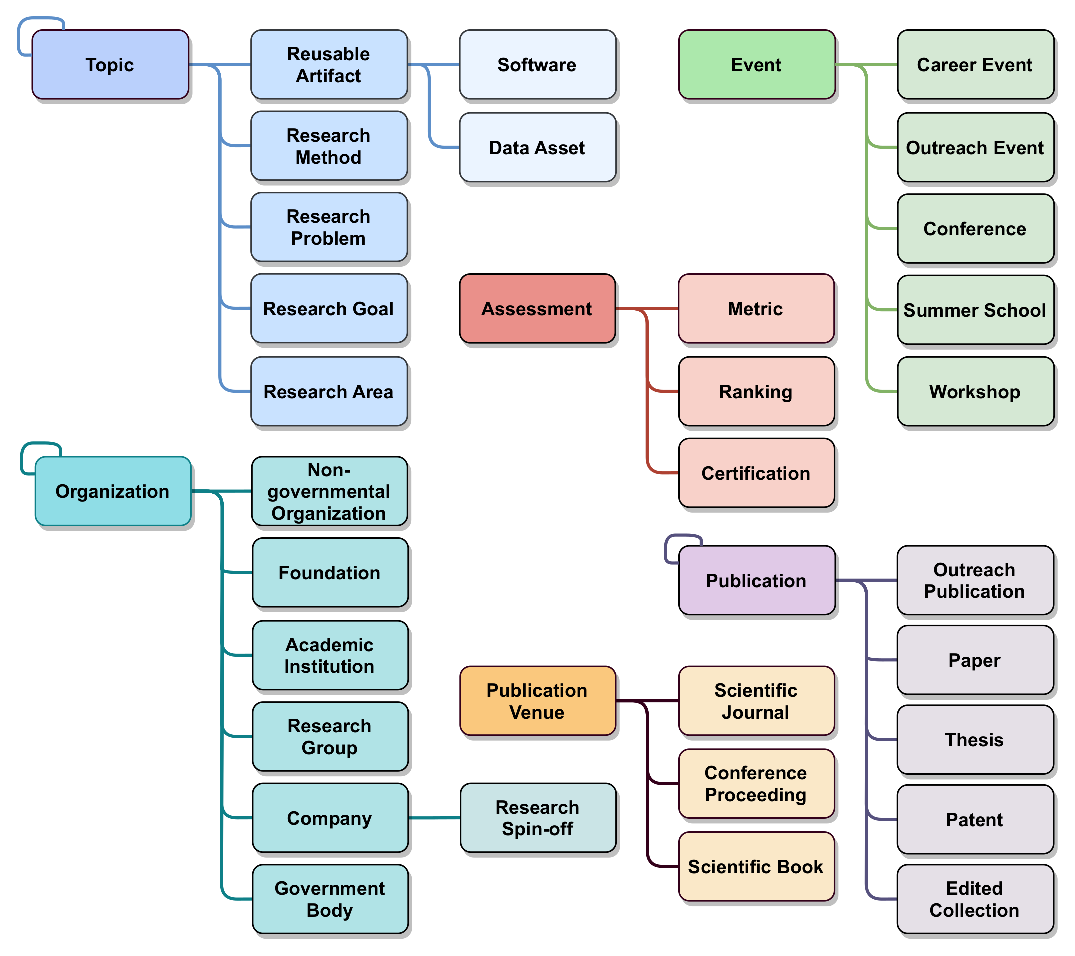
\includegraphics[width=8cm]{figures/natural-concept-hierarchy.eps}
\caption{Natural concept hierarchy} \label{natural-concept-hierarchy}
\end{figure}


All mentioned relationships in the previous descriptions of top-level concepts are captured in Figure \ref{relationship-model}. In this model, there are 3 other top-level concepts that do not have a further breakdown. We describe them as follows:


\begin{itemize}
    \item A \textit{Researcher} %top-level concept is the main actor. Researchers 
    can, e.g., be a member of organizations and can contribute to research projects and publications. %Through the \textit{Research Contribution} concept, t
    The researcher also has access to other concepts such as \textit{Event} and \textit{Publication Venue}.
    
    \item The \textit{Position} concept is used to describe possible positions or roles of a researcher within an organization.% and determine what kind of contribution does the researcher has within a project or a publication. % what about events?
    
    \item The \textit{Funding Program} concept models a source of funding for research projects, possibly assigned across multiple calls.

    \item A \textit{Project}  %refers to an organized and planned work of researchers.
    may be proposed and solved by researchers (in some positions) or organizations,  supported by funding programs, and associated with publications.% since they are one of their main outputs. The relationship with the term Position serves as the specific role of a researcher in the project.
    
    %\item The \textit{Publication Citation} top-level concept is used to describe which publication is cited by other publication and the overall relationship between publications and projects. %can a research project be cited without a publication?
    
    %\item The \textit{Publication Review} top-level concept is used to describe the role reviewer of a researcher in the reviewing process of a paper. %although this is not public info?
\end{itemize}

Note that the paths are not disambiguated, and in many cases may correspond to semantically different kinds of relationships, e.g., Researchers may provide assessments on something, but can also be assessed by other researchers.

\begin{figure}
\centering
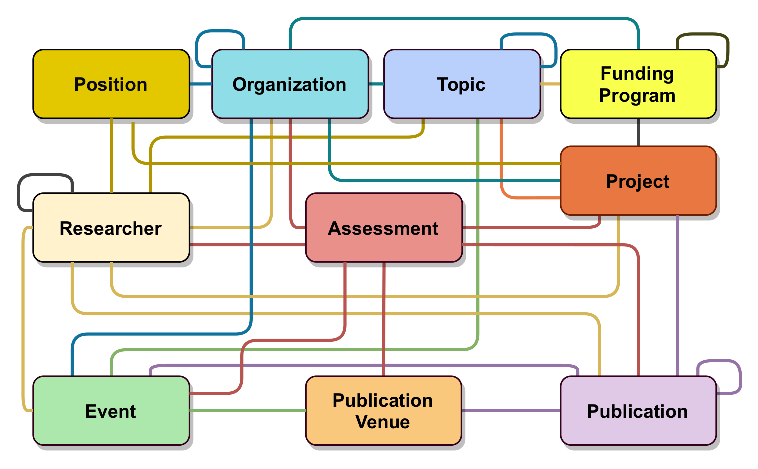
\includegraphics[width=7cm]{figures/relationship-model.eps}
\caption{High-level relationship model} \label{relationship-model}
\end{figure}



\section{Mapping the ontologies to the holistic model}
\label{section:4}


Our high-level conceptual model consists of concepts and relationships that hold between them. It can be broken down into individual elements and fragments of concepts. This is needed to map existing ontologies onto the model and to identify their coverage. For this reason, we created a spreadsheet listing concepts, their subtypes and entity-relationship paths in the first column. Then, for each examined ontology, we noted down which concept is (at least, partially) covered by which entities in those ontologies. The detailed (manual) steps can be approximately described in the form of an algorithm:

\begin{algorithm}[H]
    \caption{Ontology coverage}
    \SetKwInOut{Input}{input}
    \SetKwInOut{Output}{output}
    \SetAlgoLined
    \KwResult{Coverage table}
    \Input{Latest versions of ontologies}
    \Output{Entities}
    \ForEach{Ontology}{
        \uIf{Ontology documentation exists}{
            Check documentation\;
            \uIf{Ontology documentation has descriptive figures}{
                Use entities in figures\;
            }\uElse{
                Use entities listed in documentation\;
            }
        }
        \uElseIf{Ontology source code exists}{
            Use entities described in source code\;
        }
        \uElseIf{Paper has entity descriptions}{
            Use entities described in the paper\;
        }
    }
    \ForEach{Entity} {
        Keep only classes, their instances, object properties and datatype properties within the ontology namespace\;
    }
    \Input{Model elements}
    \Input{Entities}
    \Output{Coverage records}
    \ForEach{Entity} {
        %Match with our concepts and fragments\;
        If it is a property then also check its domain and range\;
        When in doubt, check the comments, definition or description\;
        Record the matching entities in the column of the ontology\;
    }
\end{algorithm}

In Table \ref{tab:coverage}, we show a fragment of our coverage table results. Numerical values in row \textbf{Terms covered} indicate how many concepts or relationship paths in the model are covered by the given ontology. Numeric values in column \textbf{C} indicate how many ontologies have 
%non-zero 
positive coverage for the given term from the model. Positive coverage means that an ontology concept corresponds to the naming and/or context of a term in our model, providing a similar or same semantics. In many cases, the coverage was not apparent and some manual approximation had to be made. For example, in this table, the model term \emph{Research Group} was considered to be covered by \emph{Group} in the Scholarly Ontology despite its specificity. Other cases include relationships being covered by classes, such as \emph{Researcher -- Position} vs. \emph{vivo:contributionRole}. The full coverage table of 73 model concepts and 34 ontologies can be found in our research repository, which also contains the set of CQs and other relevant resources.\footnote{\url{https://github.com/nvbach91/iga-knerd}}


\begin{table}[H]
\centering
\scriptsize
\caption{Ontology coverage -- table excerpt}
\label{tab:coverage}
\begin{tabular}{|p{2.8cm}|c|p{2.6cm}|p{2.2cm}|p{3cm}|c|}
\hline
\textbf{}                   & \textbf{C}                       & \textbf{SO}                                 & \textbf{OLOUD}            & \textbf{VIVO core}                                & ... \\ \hline
\textbf{Terms covered}      &                                    & \cellcolor[HTML]{D6DF82}\textbf{15}         & \cellcolor[HTML]{FDC57C}6 & \cellcolor[HTML]{63BE7B}34                        & ... \\ \hline
\textbf{Position}           & \cellcolor[HTML]{BDD881}\textbf{12} & :ActorRole                                  & :Role                     & :Position,\newline :Faculty Position                       & ... \\ \hline
\textbf{Position -- Project} & \cellcolor[HTML]{FFEB84}\textbf{5} & :ActorRole                                  &                           & :contributingRole                                 & ... \\ \hline \hline
\textbf{Org}               & \cellcolor[HTML]{90CB7E}\textbf{10} &                                             & :Organization             & :ResearchOrganization                             & ... \\ \hline
NGO                         & \cellcolor[HTML]{F8696B}\textbf{0} &                                             &                           &                                                   & ... \\ \hline
Foundation                  & \cellcolor[HTML]{F98971}\textbf{1} &                                             &                           & :Foundation                                       & ... \\ \hline
Academic Institution        & \cellcolor[HTML]{E9E583}\textbf{8} &                                             &                           & :Faculty, :Institute                              & ... \\ \hline
Research Group              & \cellcolor[HTML]{FBAA77}\textbf{3} & :Group                                      &                           &                                                   & ... \\ \hline
Company, Spin-off           & \cellcolor[HTML]{F98971}\textbf{1} &                                             &                           & :Company,\newline :Private Company                         & ... \\ \hline
Government Body             & \cellcolor[HTML]{F98971}\textbf{1} &                                             &                           & :GovernmentAgency                                 & ... \\ \hline
\textbf{Org -- Assessment}  & \cellcolor[HTML]{FBAA77}\textbf{2} &                                             &                           &                                                   & ... \\ \hline
\textbf{Org -- Org}        & \cellcolor[HTML]{FBAA77}\textbf{2} &                                             &                           &                                                   & ... \\ \hline
\textbf{Org -- Position}    & \cellcolor[HTML]{FFEB84}\textbf{4} &                                             & :roleAt, :role            &                                                   & ... \\ \hline
\textbf{Org -- Topic}       & \cellcolor[HTML]{F98971}\textbf{1} &                                             &                           & :hasResearchArea                                  & ... \\ \hline
\textbf{Org -- Event}       & \cellcolor[HTML]{F98971}\textbf{1} &                                             &                           &                                                   & ... \\ \hline
\textbf{Org -- Project}     & \cellcolor[HTML]{FFEB84}\textbf{6} & :ActorRole                                  &                           & :supportedBy,\newline :sponsoredBy                        & ... \\ \hline
\textbf{Org -- Fund Prog} & \cellcolor[HTML]{FFEB84}\textbf{4} &                                             &                           & :FundingOrganization                              & ... \\ \hline \hline
\textbf{Topic}              & \cellcolor[HTML]{E9E583}\textbf{7} & :Topic                                      & :Specialization           &                                                   & ... \\ \hline
Reuseable Artifact          & \cellcolor[HTML]{90CB7E}\textbf{9} & :Tool, :InformationResource                 &                           & :Dataset                                          & ... \\ \hline
Research Method             & \cellcolor[HTML]{A6D27F}\textbf{8} & :Method,  :Assertion                         &                           & :CaseStudy                                        & ... \\ \hline
Research Problem            & \cellcolor[HTML]{FDCA7D}\textbf{4} & :Proposition,\newline :ResearchQuestion &                           &                                                   & ... \\ \hline
Research Goal               & \cellcolor[HTML]{FFEB84}\textbf{5} & :Assertion, :Goal                           &                           &                                                   & ... \\ \hline
Research Area               & \cellcolor[HTML]{FFEB84}\textbf{6} & :Discipline                                 &                           & :hasResearchArea, \newline :subjectAreaOf, \newline :researchAreaOf & ... \\ \hline
\textbf{Topic -- Topic}      & \cellcolor[HTML]{FBAA77}\textbf{4} & :hasPart, :Step                             &                           &                                                   & ... \\ \hline
...                         & ...                                & ...                                         & ...                       & ...                                               & ... \\ \hline
\end{tabular}
\end{table}

% New text by VS:
The coverage table indicates that even if the roles played by researchers during their career, and the associated CQs, are numerous, the relevant concepts and relationships are mostly well covered by available ontologies.
%Our analysis took into account 34 ontologies.
Presumably, a proper (but still relatively large) subset of them might be found that would still cover all considered CQs.
For such a set of ontologies, the abstract concept-relationship paths could be instantiated by constellations of OWL entities that could become part of \emph{guidelines} for researcher data publishers. 
Possibly several alternative ontologies can be recommended for the parts of the domain where multiple of them \emph{overlap}; these are, for example, the parts dealing with publications or organizations.
More detailed criteria describing these choices in terms of ontology design patterns and their impact should be formulated.

As a likely gap in the existing ontology eco-system, we perceive, for example, the sub-domain of \emph{spin-offs}.
(In fact, even beyond the scope of the current survey, we were unable to find any ontology devoted to start-ups in general.)
Underdeveloped also seems to be the conceptualization of, e.g., \emph{funding programs} or some forms of \emph{assessment}.
In some cases, notions belonging to one `bag' are dispersed across several ontologies, lacking a unifying super-concept, e.g. a \emph{reusable artifact}.

% End of new text by VS:

%The result table gave us a comprehensive overview of related ontologies and allowed us to identify  coverage overlaps and gaps. Examples of overlaps include rows that have a value higher than 1 in column \textbf{C}. Likewise, gaps are identified based on value 0 in the same column. For each concept there can be 3 cases: (1) the concept is not covered, which is the least, (2) there is only one coverage count, and (3) there are multiple overlaps of ontologies describing essentially the same thing. If a concept in the target model is not covered, it is necessary to introduce it as a new one and connect it to the existing network if necessary. If there is only one coverage for a particular term, we need to consider whether it is an exact match or not, and then decide whether to extend it or use it as-is. The obvious problem with multiple coverage overlaps is that the selection process of the concepts for re-use will be more complicated and so proper analysis of term context and its usage purpose should be considered. Furthermore, this analysis result could be useful for identifying concepts with the same or similar semantics or context in order to link them with appropriate properties. % and use them interchangeably. 



%In case of identifying the same or very similar semantics for terms that are defined multiple times across different ontologies, it would be convenient to mark them with 

%TODO: PROPERLY FORMULATE THIS

%- Firstly, sort the ontologies by the number of covered terms and relationships descendingly, and analyze one by one to pick the best option for reuse, also considering reuse from multiple ontologies, if they complement each other well.


%- results show that there are many gaps and overlaps, this is how to deal with them:

%there are 3 cases

%1) the concept is not covered = gap, solve by proposing a new concept, example: ...

%2) there is only one coverage count, solve by analyzing that ontology and evaluate its usability. example: ...

%3) there are overlaps (more than one coverage count), solve by choosing the best option based on several criterias ..., example:



\section{Conclusions and future work}
\label{section:5}

The presented research adds to the current vivid motion around scholarly KGs the perspective of a wider scope of (senior) researcher daily activities as well as that of ontology reuse.
The comparison between a model extracted from a collection of researcher information needs and KG competence questions on one side and existing ontologies on the other side reveals that in many areas a huge number of models overlap while some others are nearly untouched.

The presented survey focused on ontologies alone.
The most imminent future work then consists in extending the survey, in an integrated manner, to actual KGs as well as to existing thesauri. 
Although any   ontology can be reused in the future, their actual usage in datasets may vary; this represents another dimension that could be added to our analysis.
We have been collecting, in parallel, links to scholarly KGs, roughly partitioned according to the concepts from the model presented in this paper. 

\medskip
\noindent
\emph{The research has been partially supported by the VSE IGS project no. 43/2020, ``Knowledge Engineering of Researcher Data (KNERD)''.}


\bibliographystyle{splncs04}
\bibliography{bib}
\end{document}
